%===============================================================================
% $Id: ifacconf.tex 19 2011-10-27 09:32:13Z jpuente $
% Template for IFAC meeting papers
% Copyright (c) 2007-2008 International Federation of Automatic Control
%===============================================================================
\documentclass{ifacconf}

\usepackage{graphicx}      % include this line if your document contains figures
\usepackage{natbib}        % required for bibliography
\usepackage{subfigure}
\usepackage{enumerate}

%===============================================================================
\begin{document}
\begin{frontmatter} 
  
% Title, preferably not more than 10 words.

%Op��o 1 de titulo
%\title{DORIS: A MOBILE ROBOT FOR MONITORING OF OFFSHORE FACILITIES - THE EMBEDDED ELECTRONICS SYSTEM\thanksref{footnoteinfo}}

%Op��o 2 de titulo
\title{THE EMBEDDED ELECTRONICS AND SOFTWARE OF DORIS OFFSHORE ROBOT \thanksref{footnoteinfo}}

\thanks[footnoteinfo]{This work is supported primarily by Petrobras S.A. and
Statoil Brazil Oil \& Gas Ltda under contract COPPETEC 0050.0079406.12.9
(ANP-Brazil R\&D Program), and in part by the Brazilian research agencies CNPq
and FAPERJ.}

\author[1]{Renan S. Freitas}
\author[1]{Marco F. S. Xaud}
\author[1]{Ighor Marcovistz}
\author[1]{Alex F. Neves}
\author[1]{Rafael O. Faria}
\author[1]{Guilherme P. S. Carvalho}
\author[1]{Liu Hsu}
\author[1]{Eduardo V. L. Nunes}
\author[1]{Alessandro J. Peixoto}
\author[1]{Fernando Lizarralde}
\author[1]{Gustavo Freitas}
\author[1]{Ramon R. Costa}
\author[2]{P{\aa}l From}
\author[3]{Mauricio Galassi}
\author[4]{Peter W. J. Derks}
\author[5]{Anders R{\o}yr{\o}y}

%%% Op��o 1 de filia��o com email
%  \address[1]{Electrical
% Engineering Department, COPPE UFRJ, Rio de Janeiro, Brazil (renan028@poli.ufrj.br, marco.fernandes@poli.ufrj.br, imtz@poli.ufrj.br, alexfneves@poli.ufrj.br, rafael.o.faria@gmail.com, guilherme\_carvalho@poli.ufrj.br,\{liu,eduardo,jacoud,fernando,gfreitas,ramon\}@coep.ufrj.br, \{eduardo,sergioln\}@smt.ufrj.br)}
% \address[2]{Mathematical Sciences and Technology Department, Norwegian
%University of Life Sciences, Oslo, Norway (pafr@umb.no)}
% \address[3]{Research and Development Center, Petrobras/CENPES,
% Rio de Janeiro, Brazil (mauricio.galassi@petrobras.com.br)}
% \address[4]{TPD RDI Mature Area Development and Increased Oil recovery (MADI) , Statoil ASA, Bergen, Norway (aroy@statoil.com)}
% \address[5]{TPD RDI Frontier Developments (FD), Statoil Brasil \'{O}leo e G\'{a}s Ltda., Rio de Janeiro, Brazil (PEDE@statoil.com)}

%% Op��o 2 de filia��o sem email
  \address[1]{Electrical
 Engineering Department, COPPE UFRJ, Rio de Janeiro, Brazil}
 \address[2]{Mathematical Sciences and Technology Department, Norwegian
University of Life Sciences, Oslo, Norway}
 \address[3]{Research and Development Center, Petrobras/CENPES,
 Rio de Janeiro, Brazil}
 \address[4]{TPD RDI Frontier Developments (FD), Statoil Brasil \'{O}leo e G\'{a}s Ltda., Rio de Janeiro, Brazil}
 \address[5]{TPD RDI Mature Area Development and Increased Oil recovery (MADI) , Statoil ASA, Bergen, Norway}

\begin{abstract}                % Abstract of not more than 250 words.
DORIS is a research project which endeavors to design and implement a mobile
robot for remote supervision, diagnosis, and data acquisition on offshore
facilities. The proposed system is composed of a rail-guided robot capable of
carrying different sensors through the inspected area. This paper presents a
general overview of the robot, and a description of the developed embedded
electronics, power supply system and software architecture. The results
with teleoperated navigation validate the concepts considered so far and
rise several challenges for future works.
\end{abstract}

\begin{keyword}
mobile robots; field robotics; embedded electronics; robotic
software architecture;
\end{keyword}

\end{frontmatter}
%===============================================================================

\section{Introduction}
The Oil \& Gas (O\&G) demand will grow rapidly in the next decades (\cite{wna})
and the need to obtain the resources from hostile environments will increase
operation costs. Also, the working conditions on offshore installations, such
as unfriendly atmosphere, heavy weather, extreme temperatures, and constrained
space are serious obstacles for O\&G
companies. In order to be competitive, companies are looking into new
technologies to be able to produce marginal fields. The
use of robotics in inspection, maintenance, and repair operations in O\&G
facilities could greatly improve efficiency, health and safety, while
decreasing operational and logistics costs.

In the specific case of Brazil, the O\&G industry is growing at a high
pace. The recent discoveries of big oil fields in the pre-salt layer off the
Brazilian coast, located 300 km from the shore at depths of 5000-7000 km
(\cite{presal}), motivates the development of an offshore  production system
with high degree of automation.

% It is highly expensive to have people working on the rig, as they
% must be housed and protected, there are costs with personal benefits such as
% health care, and the companies need to evacuate personnel quickly
% in case of an emergency.

Recent studies forecast a substantial decrease in the level of human operation
and an increase in automation on future oil fields (\cite{skourup2009robotized}).
The studies also point out the potential increase
in efficiency and productivity with robot operators, besides of the improvement in
Health, Safety, and Environment (HSE) conditions, as robots can replace humans
in tasks performed in unhealthy, hazardous, and confined areas (\cite{pal}).

The use of robotics in O\&G industry represents great technological challenges
to overcome the following aspects of offshore environments (\cite{chen}):

\begin{enumerate}[i)]
\item The \emph{atmospheric conditions} on offshore platforms are unfriendly, as
hydrocarbon resources can generate explosive and toxic gases; %The robot should be certified to operate in explosive environments.
\item \emph{Corrosive agents}: splashy salty water, salty air and corrosive chemicals;
\item \emph{Weather}: high speed wind, rain, and hail. The relative humidity is
up to 100\% and ambient temperature can vary between $-30^{\circ}$C to
$50^{\circ}$C. Possibly highly radiant heat from equipment and direct sunlight;
\item \emph{Constrained space}: complex structures for robots
such as pipes, flanges, tanks, and stairways.
\end{enumerate}

%There are different kinds of robots in the oil \& gas industry such as
%underwater pipeline repair robotic systems, robots for inspection of valve and
%lever position, gas level or leakage and acoustic anomalies monitoring, and
%robots for identify and locate fire.

Currently, the majority of the robotic systems in the O\&G industry are
used for subsea tasks, such as mapping of the seabed, and inspection and repair
of underwater equipment, risers and pipelines. However, recent research has
focused on robotic applications on the topside of oil platforms to perform
inspection and maintenance tasks, which includes valve and lever manipulation,
gas level and leakage monitoring, acoustic anomalies diagnosis, and
smoke and fire detection.
%Guilherme: Senti falta de refs para a parte do subsea

The MIMROex inspection robot (\cite{mimroex}), developed by the Fraunhofer
Institute of Manufacturing Engineering and Automation (IPA), is
capable of safely navigate in offshore environments, and autonomously execute
inspection tasks. 

Sensabot (\cite{sensabot}), a teleoperated inspection robot
developed by Carnegie Mellon University, was designed for severe weather and
atmosphere, being certified to operate in toxic, flammable and explosive
environments.



%The robot includes the following sensors:
%\begin{enumerate}[i)]
%    \item Hydrocarbon sensor
%    \item Pan/tilt/zoom camera for remote operations
%    \item Temperature sensors
%    \item Vibration sensor for pumps, motors and bearings inspection
%    \item Microphone to detect audible machinery problems
%    \item Video camera to detect obstacles
%\end{enumerate}

The SINTEF Topside Robotic System, Trondheim, Norway, is an intelligent
instrumentation system designed to enable onshore operators to monitor and
control the platform's processes (\cite{kyrkjebo2009robotic}).

%In this paper, we describe the DORIS project, which aims to develop a mobile
%robot to perform monitoring and inspection in an
%offshore platform. To this end, the system must be able to move throughout the
%monitored environment carrying different sensors, analyzing sensor data
%\emph{in loco} or storing it for a posterior analysis, and interpreting the
%results. The sensors can identify abnormalities such as intruders in restricted
%areas, abandoned objects, smoke, fire, and liquid and gas leakages.
%Furthermore, the robot is able to make machinery diagnosis, read instruments,
%and takes samples using an embedded manipulator (\cite{cba}).

DORIS is an offshore inspection and monitoring robot being developed by
COPPE/UFRJ in collaboration with Petrobras and Statoil. The robot moves
through a rail carrying different sensors, and
analyzing sensor data \emph{in loco} or storing it for posterior analysis. The
sensors can identify abnormalities such as intruders in restricted areas,
abandoned objects, smoke, fire, and liquid and gas leakages.
The robot has an embedded manipulator, which enables machinery vibration
diagnosis, instruments reading, and sample taking (\cite{cba}).

In this paper, we present a general overview of the DORIS robot, and a detailed
description of the embedded electronics, power supply system and software
architecture.
%This text is organized as follows: a general overview of the robot and its main
%challenges are presented in Section \ref{sec:general_overview}, detailed
%descriptions of the embedded electronics, the vehicle support system, power
%supply system, and software architecture are taken in
%Sections \ref{sec:electronics_overview}, \ref{sec:powersupply_overview}, and
%\ref{sec:software} respectively.
%In Section \ref{sec:results}, preliminary results are shown, and concluding
%remarks are drawn in Section \ref{sec:conclusions}.

\section{General Overview}\label{sec:general_overview}

%The DORIS robot contains a manipulator arm, cameras, microphones, and gas,
%vibration and temperature sensors. 
DORIS moves through a rail
and both of them are based on a modular concept.
Additional robot modules can be annexed to include extra sensors, and the rail
track can be modified by adding or replacing rail segments, thus enabling
operation in different areas of the platform. Figure~\ref{fig:DORIS-overview}
illustrates the operation in a production plant.

The robot is controlled autonomously or by teleoperation. Task managing
can be either in automatic (programmed using a mission interface) or manual
mode (real-time remote operation). The teleoperation and monitoring
capabilities guarantee online access to the embedded sensors, providing
information of the surrounding environment and the robot operating
conditions with real-time processing.


\begin{figure}[ht]
\centering
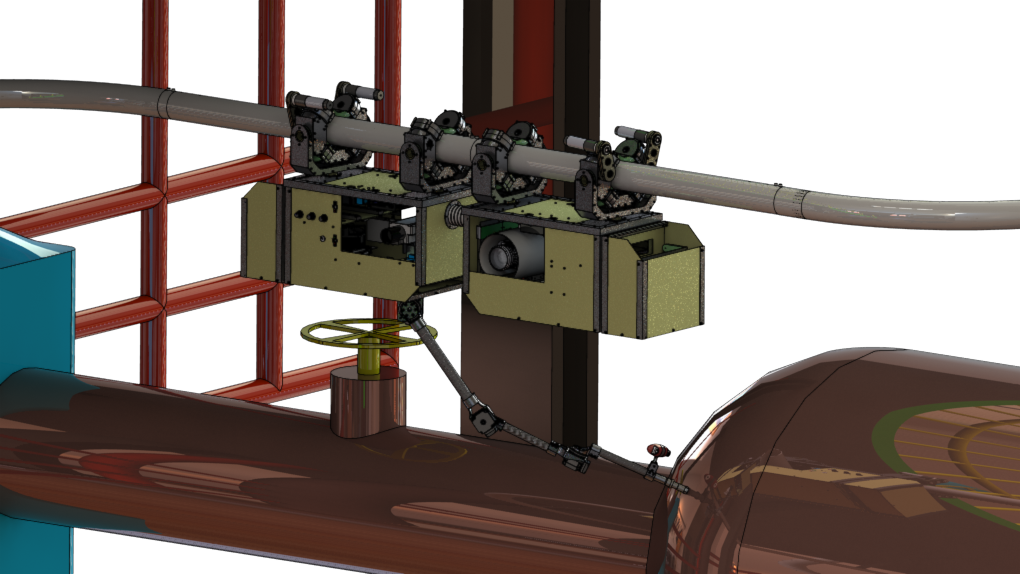
\includegraphics[width=8.4cm]{figs/cenario5.png}
\caption{Illustration of operation in a production plant.}
\label{fig:DORIS-overview}
\end{figure}

DORIS description can be split into five fields: mechanics, signal
processing, electronics, power supply and software.

%-------------------------------------------------------------------------------------------------------------------------
%ELECTRONICS
%-------------------------------------------------------------------------------------------------------------------------
% The electronics subsystem is responsible for providing embedded computational
% support for the robot control, signal processing, task managing, and local and
% remote communication. The device motion is controlled through drivers that can
% receive position, velocity, or current setpoints. The embedded electronics has
% two printed circuit boards for the vehicle support system: energy distribution
% and monitoring, basic failure detection, emergency handling and devices'
% control.

%-------------------------------------------------------------------------------------------------------------------------
%POWER SUPPLY
%-------------------------------------------------------------------------------------------------------------------------
% The power supply system uses military-class lithium-ion batteries, which have
% small size and high energy capacity. In the first prototype of DORIS, four
% batteries are used to power the motors and two to power the other electronics
% components.


%-------------------------------------------------------------------------------------------------------------------------
%SOFTWARE
%-------------------------------------------------------------------------------------------------------------------------
% The main objective of the software subsystem is to allow the implementation of
% high- and low-level control of the robot. The tools used to develop DORIS
% software architecture must consider two important factors: they have to be
% commercially available, and provide modular functionalities. These requirements
% led to the adoption of Qt as the graphical interface framework ~\cite{qt},
% Robot Operating System (ROS) as the communication middleware ~\cite{ros}, and
% Ubuntu as the operating system.
%
% The software provides autonomous control (programmed tasks) and remote control
% through a Graphical User Interface (GUI) in the Host Control Base (HCB)
% computer. The HCB is composed of a set of processes running in parallel
% denominated ROS nodes, which can communicate with each other. To deal with this
% environment, a new software architecture called Robot Package Software is
% proposed, dividing the software into tools (graphical windows) and components
% (processing and communication unities), and grouping them into a dynamic
% library.

%-------------------------------------------------------------------------------------------------------------------------
%Mechanics
%-------------------------------------------------------------------------------------------------------------------------
The \emph{mechanics} comprises the robot modules, their coupling joints, and
the rail. The mechanical design allows the robot to move smoothly in a 3D space
and to make a full stop anywhere on the track. It incorporates the use of gimbals
containing traction and guide wheels which surround a tubular rail. Since the
rail in an offshore facility may be as long as kilometers, it
is designed to be as simple as possible to keep its cost to a minimum, while the
design complexity is left to the robot. The use of two sets of gimbals provide
mechanical compliance with rail curvatures, and smoothness of the robot's base
motion.


%Considering the severe corrosion and weather conditions in offshore
%environments, the choice of materials is imperative for the success of the
%mechanical project and certified solutions must be considered if available.

The robot is composed of two modules in default configuration, has an estimated
total weight of 50 kg, and can reach a maximum speed of 1 m/s.

%-------------------------------------------------------------------------------------------------------------------------
%DSP
%-------------------------------------------------------------------------------------------------------------------------
DORIS has the following signal processing capabilities::
\begin{enumerate}[i)]
  \item \emph{Video}: use
of multiple cameras (visible-light, infrared, panoramic, and stereo) to detect
video anomalies such as abandoned objects, smoke, fire, and fluid leakage;
  \item \emph{Audio}: detection of anomalies of impulsive nature, such as
an explosion, and machinery diagnosis based on energy and pitch
(fundamental frequency) signatures using a single or an array of microphones;
  \item \emph{Vibration analysis}: use of accelerometers to diagnose the operation mode
of rotating machines, performing possible fault classification, such as
 misalignment and unbalancing operation;
  \item \emph{Gas sensor}: identification of gas level and leakages;
  \item \emph{Mapping}: environment 3D model with a laser scanner.
\end{enumerate}

The main idea of all these signal processing features is to make the robot
perform an initial reference round on the closed rail track, being manually
validated by a system operator. In the subsequent rounds, all signal processing
algorithms compare the newly acquired signals with the reference data to detect
any form of anomaly, as indicated above. Once an anomalous behavior is
detected, an alarm is flagged to the system, which stores all associated data
for immediate or future diagnosis.
%round ou lap?

A detailed presentation of the mechanical and signal processing systems of
DORIS can be found in \cite{OTC} and \cite{cba}.

%-------------------------------------------------------------------------------------------------------------------------
%OTHER CHALLENGES
%-------------------------------------------------------------------------------------------------------------------------
Considering the robot functionalities and the aggressive offshore environment,
several challenges should be addressed. Regarding the robustness and safety
required to operate in classified areas, the robot must be: sealed against
water and particles, resistant to a wide temperature range, protected from
impact and vibration, electrically shielded to avoid explosion by ignition, and
equipped with a monitoring system. Another concern is that the embedded
computers must run heavy signal processing algorithms, requiring high computational power. On the other hand,
the power supply system must efficiently provide power and maintain a low level of
power consumption.

%Further complications arise because the system is designed to move in confined
%and cluttered environments, and must have efficient wireless communication with
%operators, providing online information of sensors data.

%Temperatures in offshore facilities can
%vary between $-30^{\circ}$C to $50^{\circ}$C, relative humidity can reach
%100\%, and there may be splash water, salty air, storms, and high extensive
%corrosion ~\cite{graf2007mobile}.

\section{Embedded Electronics}\label{sec:electronics_overview}
The embedded electronics (EE) is composed of a local central computer,
a remote operation base and the following subsystems: communication, actuation,
data acquisition, and vehicle support system (VSS).

The embedded computer is the robot decision center, and it is in charge
of:
heavy data processing, data
storing, data management, control of the actuation system, and teleoperation.
The computer is composed of a high performance Intel\textregistered
Core\texttrademark i7 microprocessor embedded in a PCIe/104 form factor board,
RAM cards and an SSD (\emph{solid-state drive}) card. The use of these
components enables an easy expansion of the system.

The \emph{remote base} is the user workstation in the offshore facility
through where DORIS can be teleoperated. It is composed of a radio
joystick, a Wi-Fi access point and a computer system with a graphical user
interface (GUI).

% ALEX! The GUI includes buttons for DORIS control, buttons for device remote on/off, monitoring reports of current/voltage/temperature/failure, among other functions.

The \emph{communication system} comprises the data traffic within the robot and between the robot and the remote base. This system is composed of:

\begin{enumerate}[i)]
  \item \emph{Local Gigabit Ethernet} network for heavy data real-time traffic within the robot, such as video, audio and commands from/to the computer;
  \item \emph{Controller Area Network} (CAN) bus for control commands to the actuation system;
  \item \emph{Wireless technologies}: DORIS can be remotely operated via Wi-Fi IEEE 802.11n or via 2.4/5.0 GHz radio joystick, upon Wi-Fi absence or failure.
      % There are two Wi-Fi access points: one placed on the robot and another one at the remote base (also, one radio transceiver on the robot and another on the base).
\end{enumerate}

The Ethernet network has a star topology
centralized by an OSI-Layer 2 Switch, and connects the computer, Ethernet
peripheral devices (such as cameras), a local Wi-Fi access point and the
vehicle support system (VSS). This network topology allows easy expansion of
the Ethernet network for additional robot modules. 

The \emph{actuation system} comprises the CAN bus and the \emph{traction
subsystem}, which is composed of four controller drivers (Maxon EPOS2
70/10) and four motor packs, each containing a high power 200 W EC-4pole Maxon
brushless motor, an encoder and a planetary gearhead with 21:1 ratio. DORIS
traction is commanded via CAN bus (computer to drivers), which provides
reliability and appropriate speed to this application
(\cite{can}). The interface between the computer and the CAN bus is a
PCI/104-Express board with a galvanic opto-isolator to minimize interference on
the rest of the EE system, since the motors generate significant conductive
noise.

% Gustavo: Falar do Watchdog do alex.
% Guilherme: Nao sera falado agora

The \emph{data acquisition system} collects image, video, and audio data from
the environment. It is composed of a fixed camera, an infrared thermal camera
for thermal map and temperature measurement, a \emph{fisheye} camera, two
stereoscopic webcams (with embedded microphone), and an USB Inertial Measurement
Unit (IMU).

An overall scheme of DORIS EE system is shown in Fig.~\ref{fig:EE-Communications}.

\begin{figure}
\centering
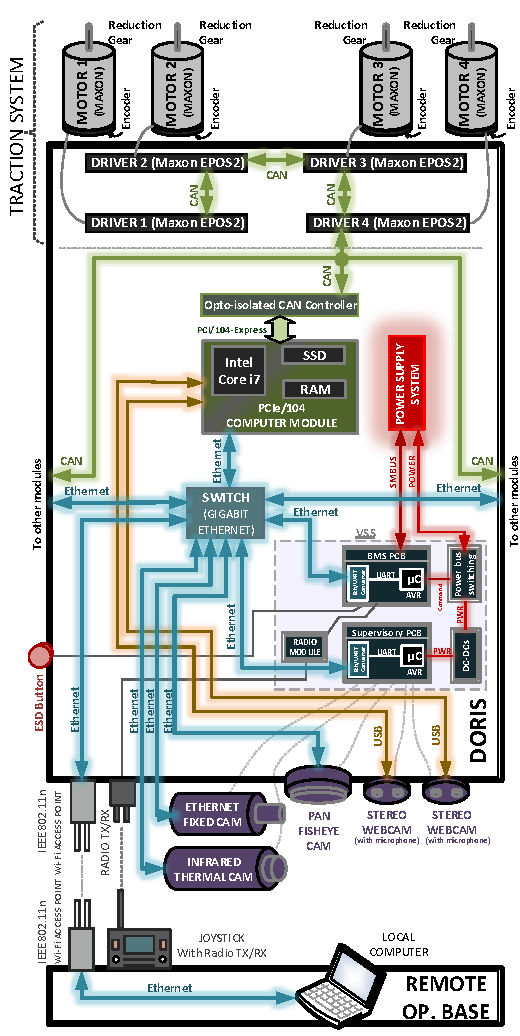
\includegraphics[width=8.4cm]{figs/EE-Communications-Geral.pdf}
\caption{Overall scheme of DORIS EE system.}
\label{fig:EE-Communications}
\end{figure} 

\subsection{Vehicle Support System}\label{sec:VSS}

The \emph{Vehicle Support System (VSS)} (\cite{MARIUS}) is composed of
microcontroller based \emph{printed circuit boards} (PCBs) designed for:

\begin{enumerate}[i)]
    \item \emph{Failure detection} achieved by the monitoring of devices'
    current/voltage and module temperature/humidity;
    \item \emph{Devices protection} against overcurrent by fuses and
    solid-state relays;
    \item \emph{Energy distribution and monitoring};
    %achieved by the \emph{Battery Management System (BMS)}. Each battery pack is monitored via \emph{System Management Bus} (SMBUS), which reads battery status, voltage, current, temperature, state of charge, and other variables. With this information, the VSS provides adequate power balance to both electronics and motor , and may reconfigure the power supply distribution in case of failures or extreme situations;
    \item \emph{Emergency handling}: the robot can be turned on/off using a physical
    \emph{emergency shutdown (ESD)} button or via radio. 
  \end{enumerate}

DORIS VSS is part of EE hardware (Fig.~\ref{fig:EE-Communications}), and
includes three types of PCBs: supervisory, Battery Management Sytem (BMS) and
Power Bus Switching (PBS).

The \emph{supervisory PCB} is composed of an ATMEL AVR AT90CAN64
microcontroller and several sensors. Its main monitoring functionalities are to
read: supply currents of peripheral devices (hall-effect sensors and a 16-ch
ADC); the module's temperature/humidity (I$^{2}$C SHT71 sensor); and the supply
voltages (AVR embedded ADC). The AVR manages the collected data, report it
periodically to DORIS computer via Ethernet, and locally detect or react to
faulty situations. Since Ethernet is not an available interface in this AVR
model, an UART-to-Ethernet converter is used. The local fault detection is done
by AVR pre-programmed algorithms, which reacts to protect devices against
overcurrent/overvoltage by commanding the open/close state of
solid-state relays, hence turning off the devices. All these AVR
functionalities can also be commanded by the remote operator. 

The \emph{BMS PCB} is in charge of managing the power supply system. It
communicates with the batteries via \emph{System Management Bus} (SMBUS) and
has a connection with the \emph{PBS PCB}. SMBUS is the interface of
the telemetry system embedded in DORIS battery model. This system collects
important information from the batteries, such as temperature, voltage, current
and state of charge. The BMS PCB periodically reports all data to DORIS computer
via Ethernet with the UART-to-Ethernet converter.

The \emph{PBS PCB} contains high power solid-state relays (20
A), which can be commanded from the \emph{BMS PCB} to distribute the power of each
battery pack. The decisions about the best power balancing are based primarily
on data collected via SMBUS.

\section{Power supply system}\label{sec:powersupply_overview}
The power supply system is responsible for the safe, reliable, and
efficient electric power distribution for DORIS devices. The electric power is
supplied by high energy density military lithium ion batteries, which comes
with an intrinsically safety circuit for protection against short-circuits and
heating. Each battery pack has a capacity of 10 Ah when delivering 24 Vdc.
According to mechanical constraints, each DORIS module admits a maximum of four battery packs, weighing 1.4 kg each.

%As \cite{verma2004real} highlights, field robots often
%operate in environments where human intervention is expensive, slow,
%unreliable, or impossible. Therefore, it is essential to monitor their behavior
%through the BMS PCB, which reads the batteries data
%via SMBus protocol as described in section \ref{sec:VSS},
%so that faults may be addressed before they result in dangerous failures.

In order to avoid electromagnetic interference (EMI) and conductive noise
interference caused by the robot motors, the system works with two separate power
buses, each one using two 24 Vdc/20 Ah batteries connected in parallel. One bus
is dedicated to power the motors and the other power all the electronic
devices.

DC-DC converters are employed to create different and stable voltage levels: 24
Vdc, 12 Vdc and 5 Vdc. To improve power supply
protection, fuses protect the system from undesired peaks, and buttons allow power
buses to be separately turned on/off.

Since DC batteries are the power source of the robot, there is no need of
capacitors to correct delays between current and voltage. However, a capacitor
bank would allow additional energy to the motors. The the capacitor bank must
have at least 400 to 500 $\mu F/A$ (\cite{capacitor}). In the case of DORIS, as
each motor may require a peak current of 20 A, a capacitor bank dedicated for
each driver would need between 8000 and 10000 $\mu F$, 36 V (maximum operating
voltage). Also, the capacitors should have low equivalent series resistance and
should be located as close as possible to the noise source, namely the motors.

The batteries are connected to the \emph{PBS PCB}, which has solid
state relays able to link each battery to any of the two power buses and diodes
to avoid back flow current, for safety. This is done by switching both the
positive and the negative poles of a battery into a power bus simuntaneously.
The \emph{PBS PCB} logic is implemented on the \emph{BMS PCB}, responsible for
commanding the relays in order to guarantee a safe and robust
operation. 



%\begin{figure}[ht]
%\centering
%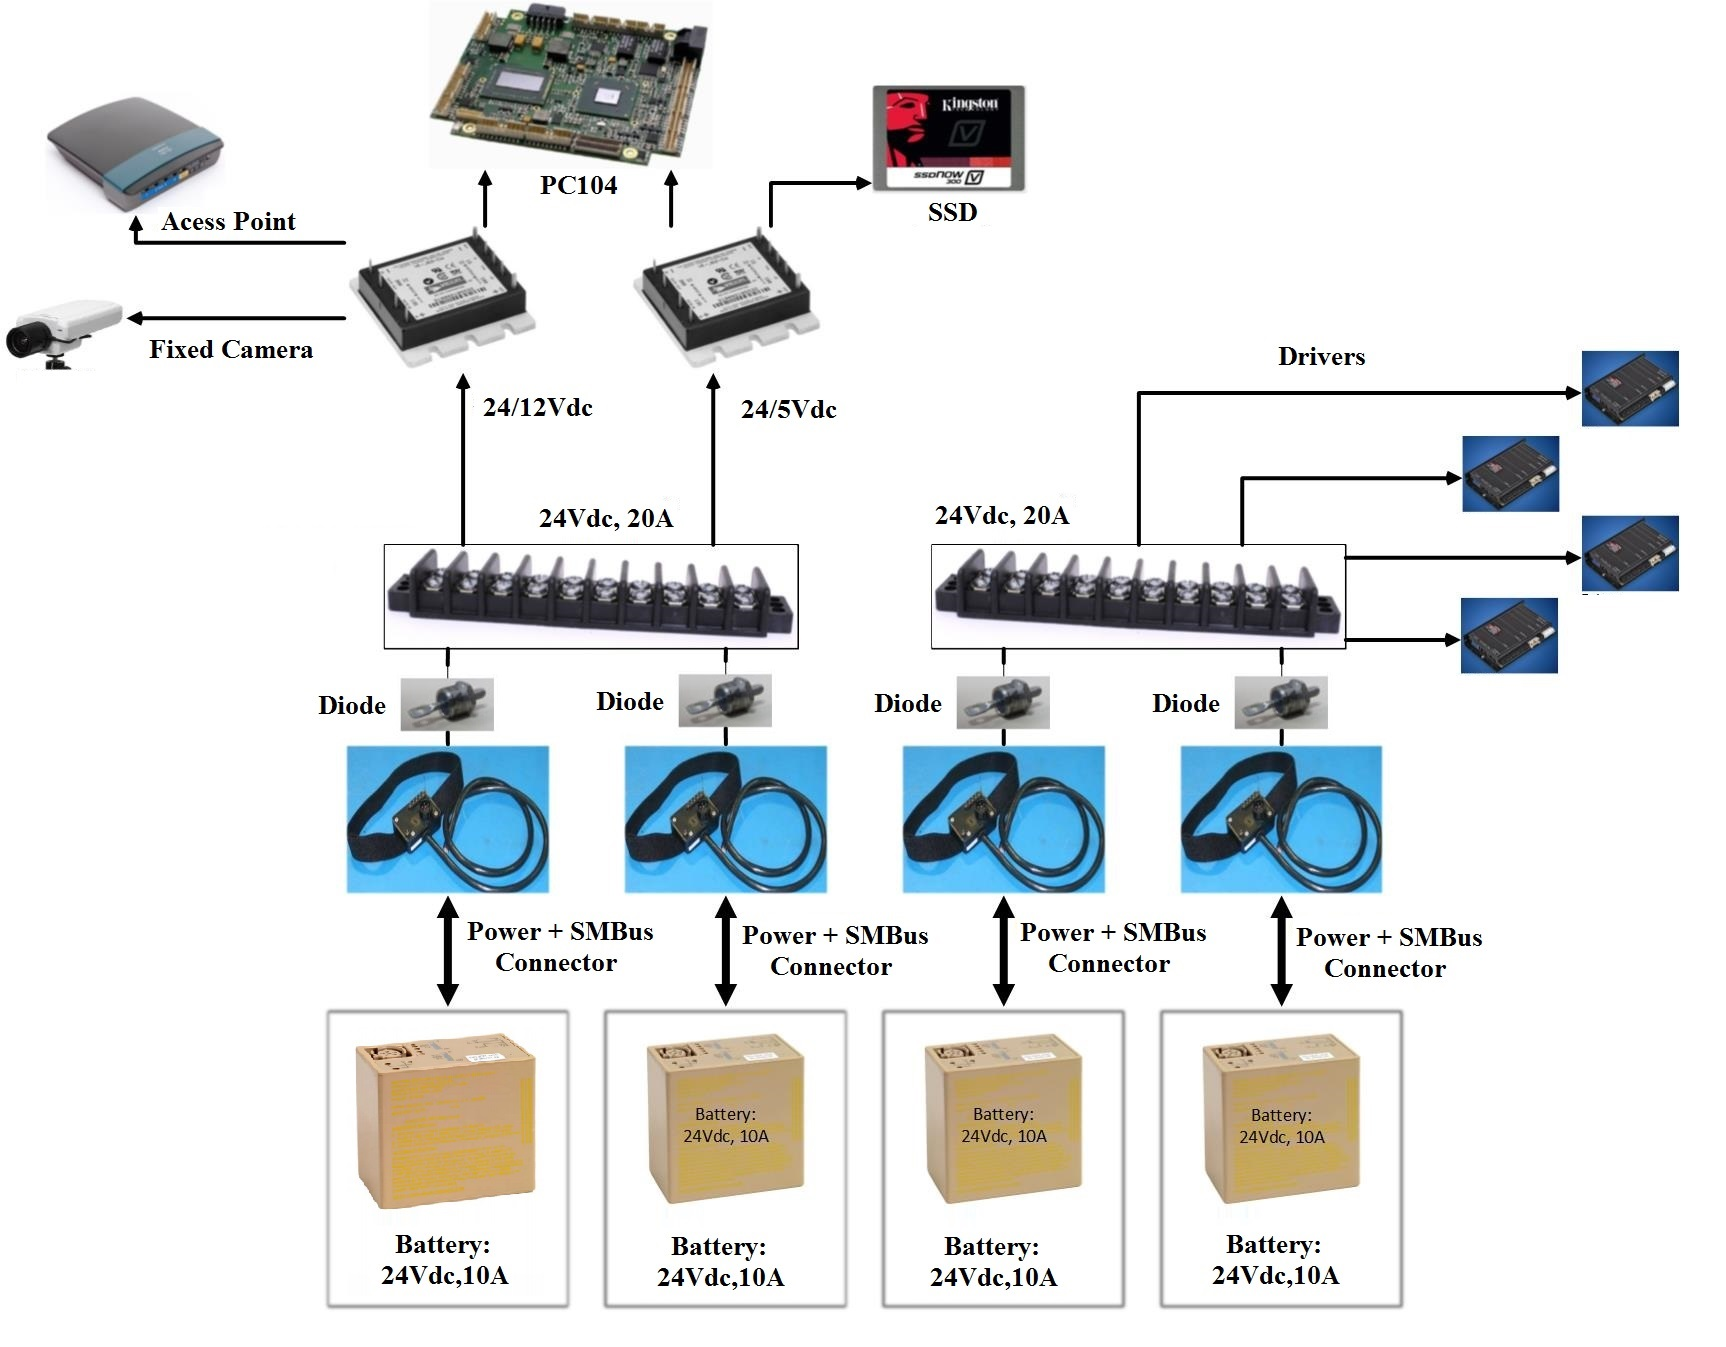
\includegraphics[width=1\columnwidth]{figs/DiagramaSAM.jpg}
%\caption{DORIS power supply architecture.}
% \label{fig:DiagramaSAM}
%\end{figure}

%Considering this, new challenges arise in order to improve the features of
%the system.
%Gustavo: Frase muito largada!

\section{Software System}\label{sec:software}

The software architecture allows the implementation of high and low level
control of the robot. It considers two important factors: tools are open-source
and provide modular functionalities. These requirements led to the adoption of
Qt as the graphical interface framework (\cite{qt}), Robot Operating System
(ROS) as the communication middleware (\cite{ros}), and Linux/Ubuntu as the
operating system.

The software provides autonomous control (programmed tasks) and remote control
through a GUI in the Host Control Base (HCB)
computer. In both computers (robot and HCB), a set of processes, denominated \emph{ROS
nodes}, runs in parallel and can communicate with each other.

To deal with this specification, a software framework that works over the ROS
environment is proposed, named \emph{Robot Package Software}. It is based on
\emph{Tools} (graphical windows) and \emph{Components} (processing and
communication unities) grouped into \emph{Robot Packages} (which are dynamic
libraries), and also the \emph{ROS node} \emph{Robot GUI} (that can load those
\emph{Robot Packages} on run-time). The \emph{Components} that deal
with hardware should run on the robot's embedded PC, while others that interact
with \emph{Tools} should run on the HCB. \emph{Components} communicate with each
other through ROS, thus allowing the HCB to view and control the robot.
Fig.~\ref{fig:robotgui} shows the robot control through the Robot GUI.

\begin{figure}[!h]
\centering
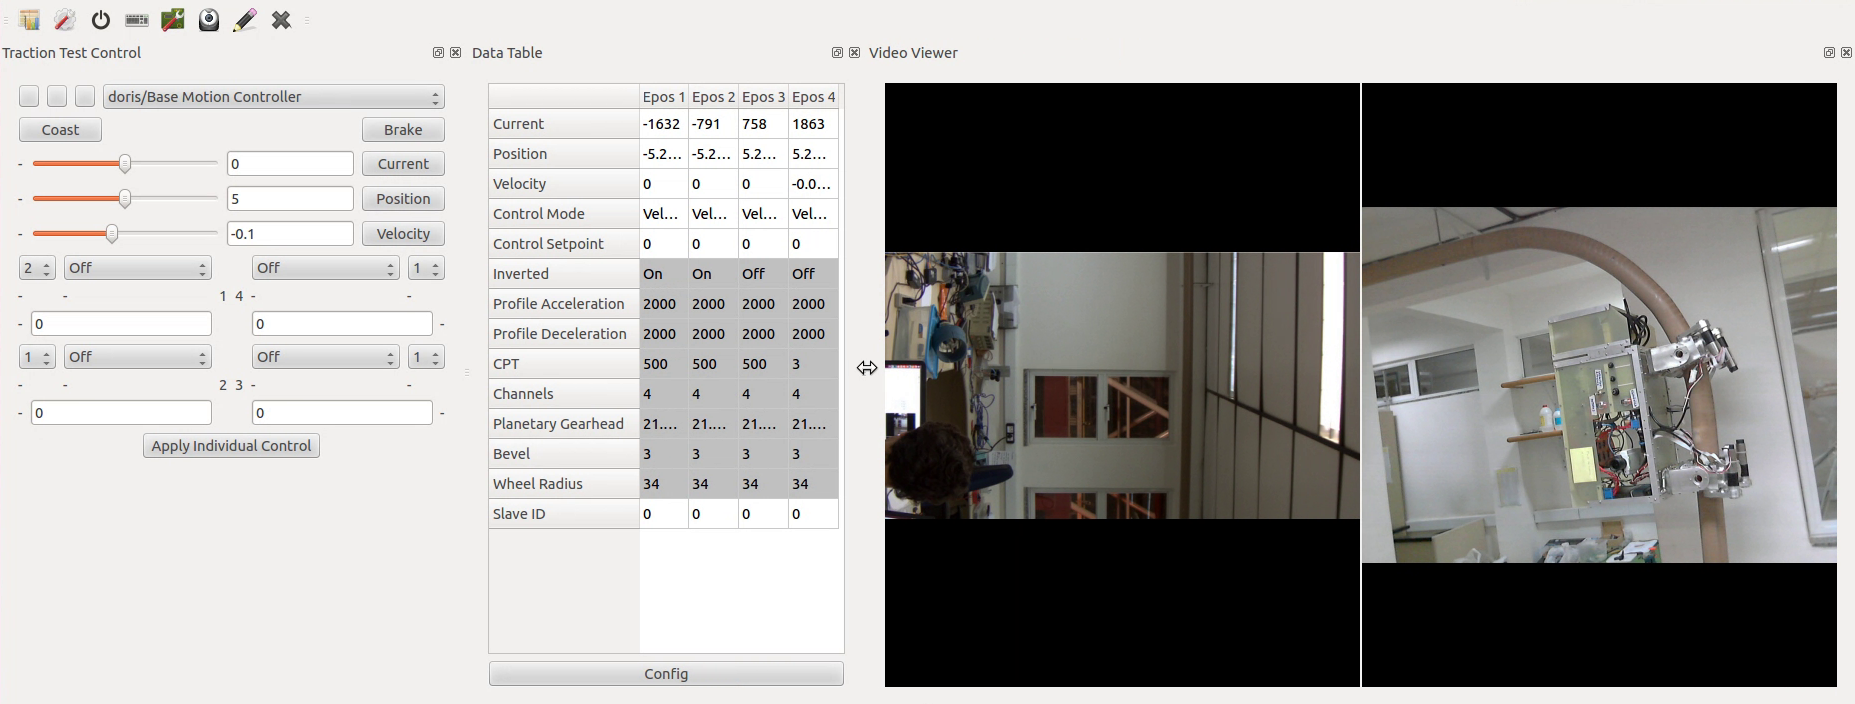
\includegraphics[width=8.4cm]{figs/robotgui2.png}
\caption{Robot GUI.}
\label{fig:robotgui}
\end{figure}

\emph{Robot Packages} can be derived from other \emph{Robot Packages}, so that
\emph{Components} and \emph{Tools} from the derived package can interact with
the ones on the base package. Two \emph{Robot Packages} have been defined: the
\emph{General Package} and the \emph{DORIS Package}, derived from the first.
The \emph{General Package} contains generic \emph{Components} and \emph{Tools}
related to video, audio, data table, gamepad, and devices configuration that can
be used on other robotic systems. The \emph{DORIS Package} is more specific to
DORIS and deals with its hardware and functionalities: it has just one
\emph{Tool} to control the 4 motors; and \emph{Components} acquire video from
an IP camera, interface with the CAN bus to control the motors, and communicate
with the PCB boards through a serial bus.

Within the ROS environment any message can be logged during the robot
operation, including audio, video, sensors, control and motors data. The
recording and playback of the logs is not integrated in the \emph{Robot GUI}
yet, so it's done by ROS commands. Still, the data being played can be viewed
in the \emph{Robot GUI}.

A robot 3D model based on ROS \emph{Unified Robot Description Format} (URDF),
which is an XML format to represent a robot model, is presented in Fig.~\ref{fig:rviz}.
The 3D model, which includes the rail and the robot system, is integrated in the GUI and can be
visualized using RVIZ (a ROS tool). Thus, the robot motion can be visualized
in the GUI and the operator can control the robot in the 3D environment by
marking a desired setpoint position on the interface.

\begin{figure}[!h]
\centering
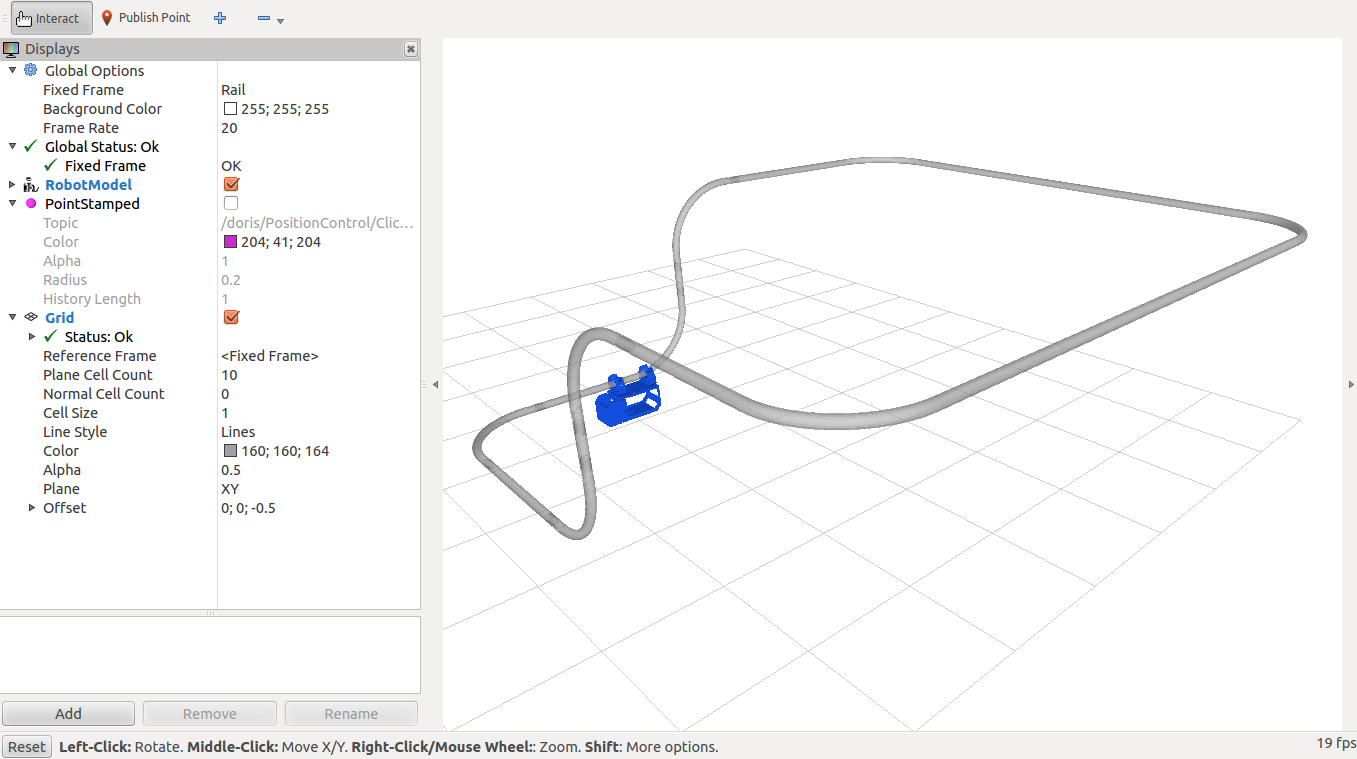
\includegraphics[width=8.4cm]{figs/rviz.png}
\caption{Robot system 3D model.}
\label{fig:rviz}
\end{figure}

%A Web tool is also proposed to remotely control DORIS using a standard internet
%browser with \emph{javascript} support (Fig.~\ref{fig:teleop}). The webtool is
%based on \emph{rosbridge} and \emph{javascript} libraries \emph{roslibjs},
%\emph{ros2js} and \emph{ros3djs}.

%\begin{figure}[!h]
%\centering
%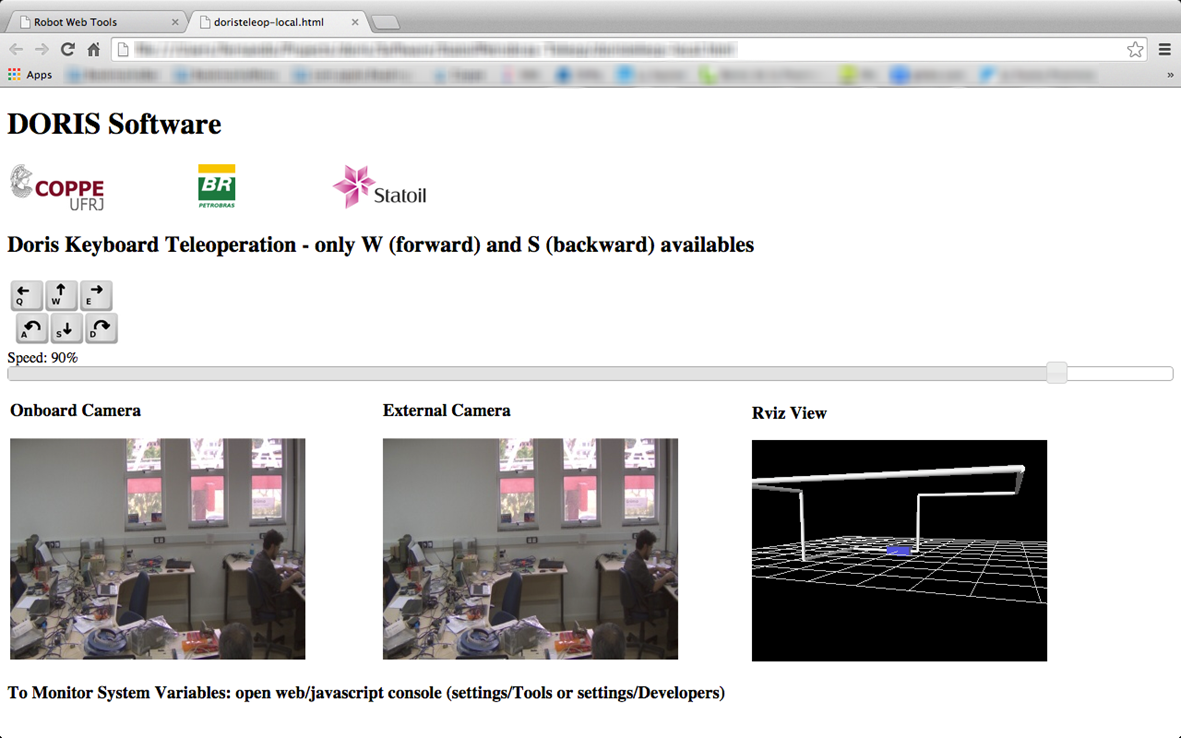
\includegraphics[width=8.4cm]{figs/teleop.png}
%\caption{Web tool to remotely control DORIS using a standard internet browser.}
%\label{fig:teleop}
%\end{figure}


\section{Experimental tests and results}\label{sec:results}
A prototype named \emph{Single Autonomous Module} (SAM) was built to verify the
proposed concepts. In addition, some VSS functionalities were
individually tested, but not yet fully integrated with SAM. Subsections
\ref{sec:SAM_tests} and \ref{sec:VSS_tests} below detail the executed tests.

\subsection{Single Autonomous Module (SAM)}\label{sec:SAM_tests}
SAM (Fig.~\ref{fig:SAM2}) is a single module composed of an AXIS ethernet fixed
camera, two USB Minoru stereoscopic Webcams, an IMU, a Cisco wireless router,
four Maxon motor packs and Maxon EPOS2 drivers, a PCIe/104 with Intel Core i7
computer module, 4GB DDR3 RAM, 240GB SSD (Kingston), and a dual-channel
opto-isolated PCI-express CAN interface.

SAM was tested in horizontal and vertical motion on a closed rail made of
straight and curved PVC tubes. The curved segments are straight tubes of 1 m
bent by $90^{\circ}$, resulting in a curvature of approximately 630 mm. The
complete track has 23 m length and comprises all the possible robot motion
types. The rail was installed in the GSCAR laboratory, in COPPE/UFRJ (Brazil),
and SAM was able to fully move throughout the entire track. 

The SAM's electronics power bus uses 14 AWG wires (up to 15 A), and the motors
power bus uses 12 AWG wires (up to 21 A). The \emph{power
bus switching PCB} was not yet implemented, thus diodes were welded on the
positive pole of each battery and then this pair of cables was connected to a
screw block linking the positive poles on a specific bus. The same was done with
the negative poles in another area of the screw block, creating a parallel
connection. After the screw block, a 20 A cable is connected to the input of
the DC-DC converters, and their output is delivered to the corresponding device.

Concerning electronics, power supply, and software, the first objectives of SAM were to test the following concepts:
\begin{enumerate}[i)]
  \item \emph{Electronics}: sensor integration and communication system;
  \item \emph{Power supply}: independent buses for motors and electronics
  devices, batteries robustness, and autonomy;
  \item \emph{Software}: teleoperation and user interface.
  \end{enumerate}

\begin{figure}[!h]
\centering
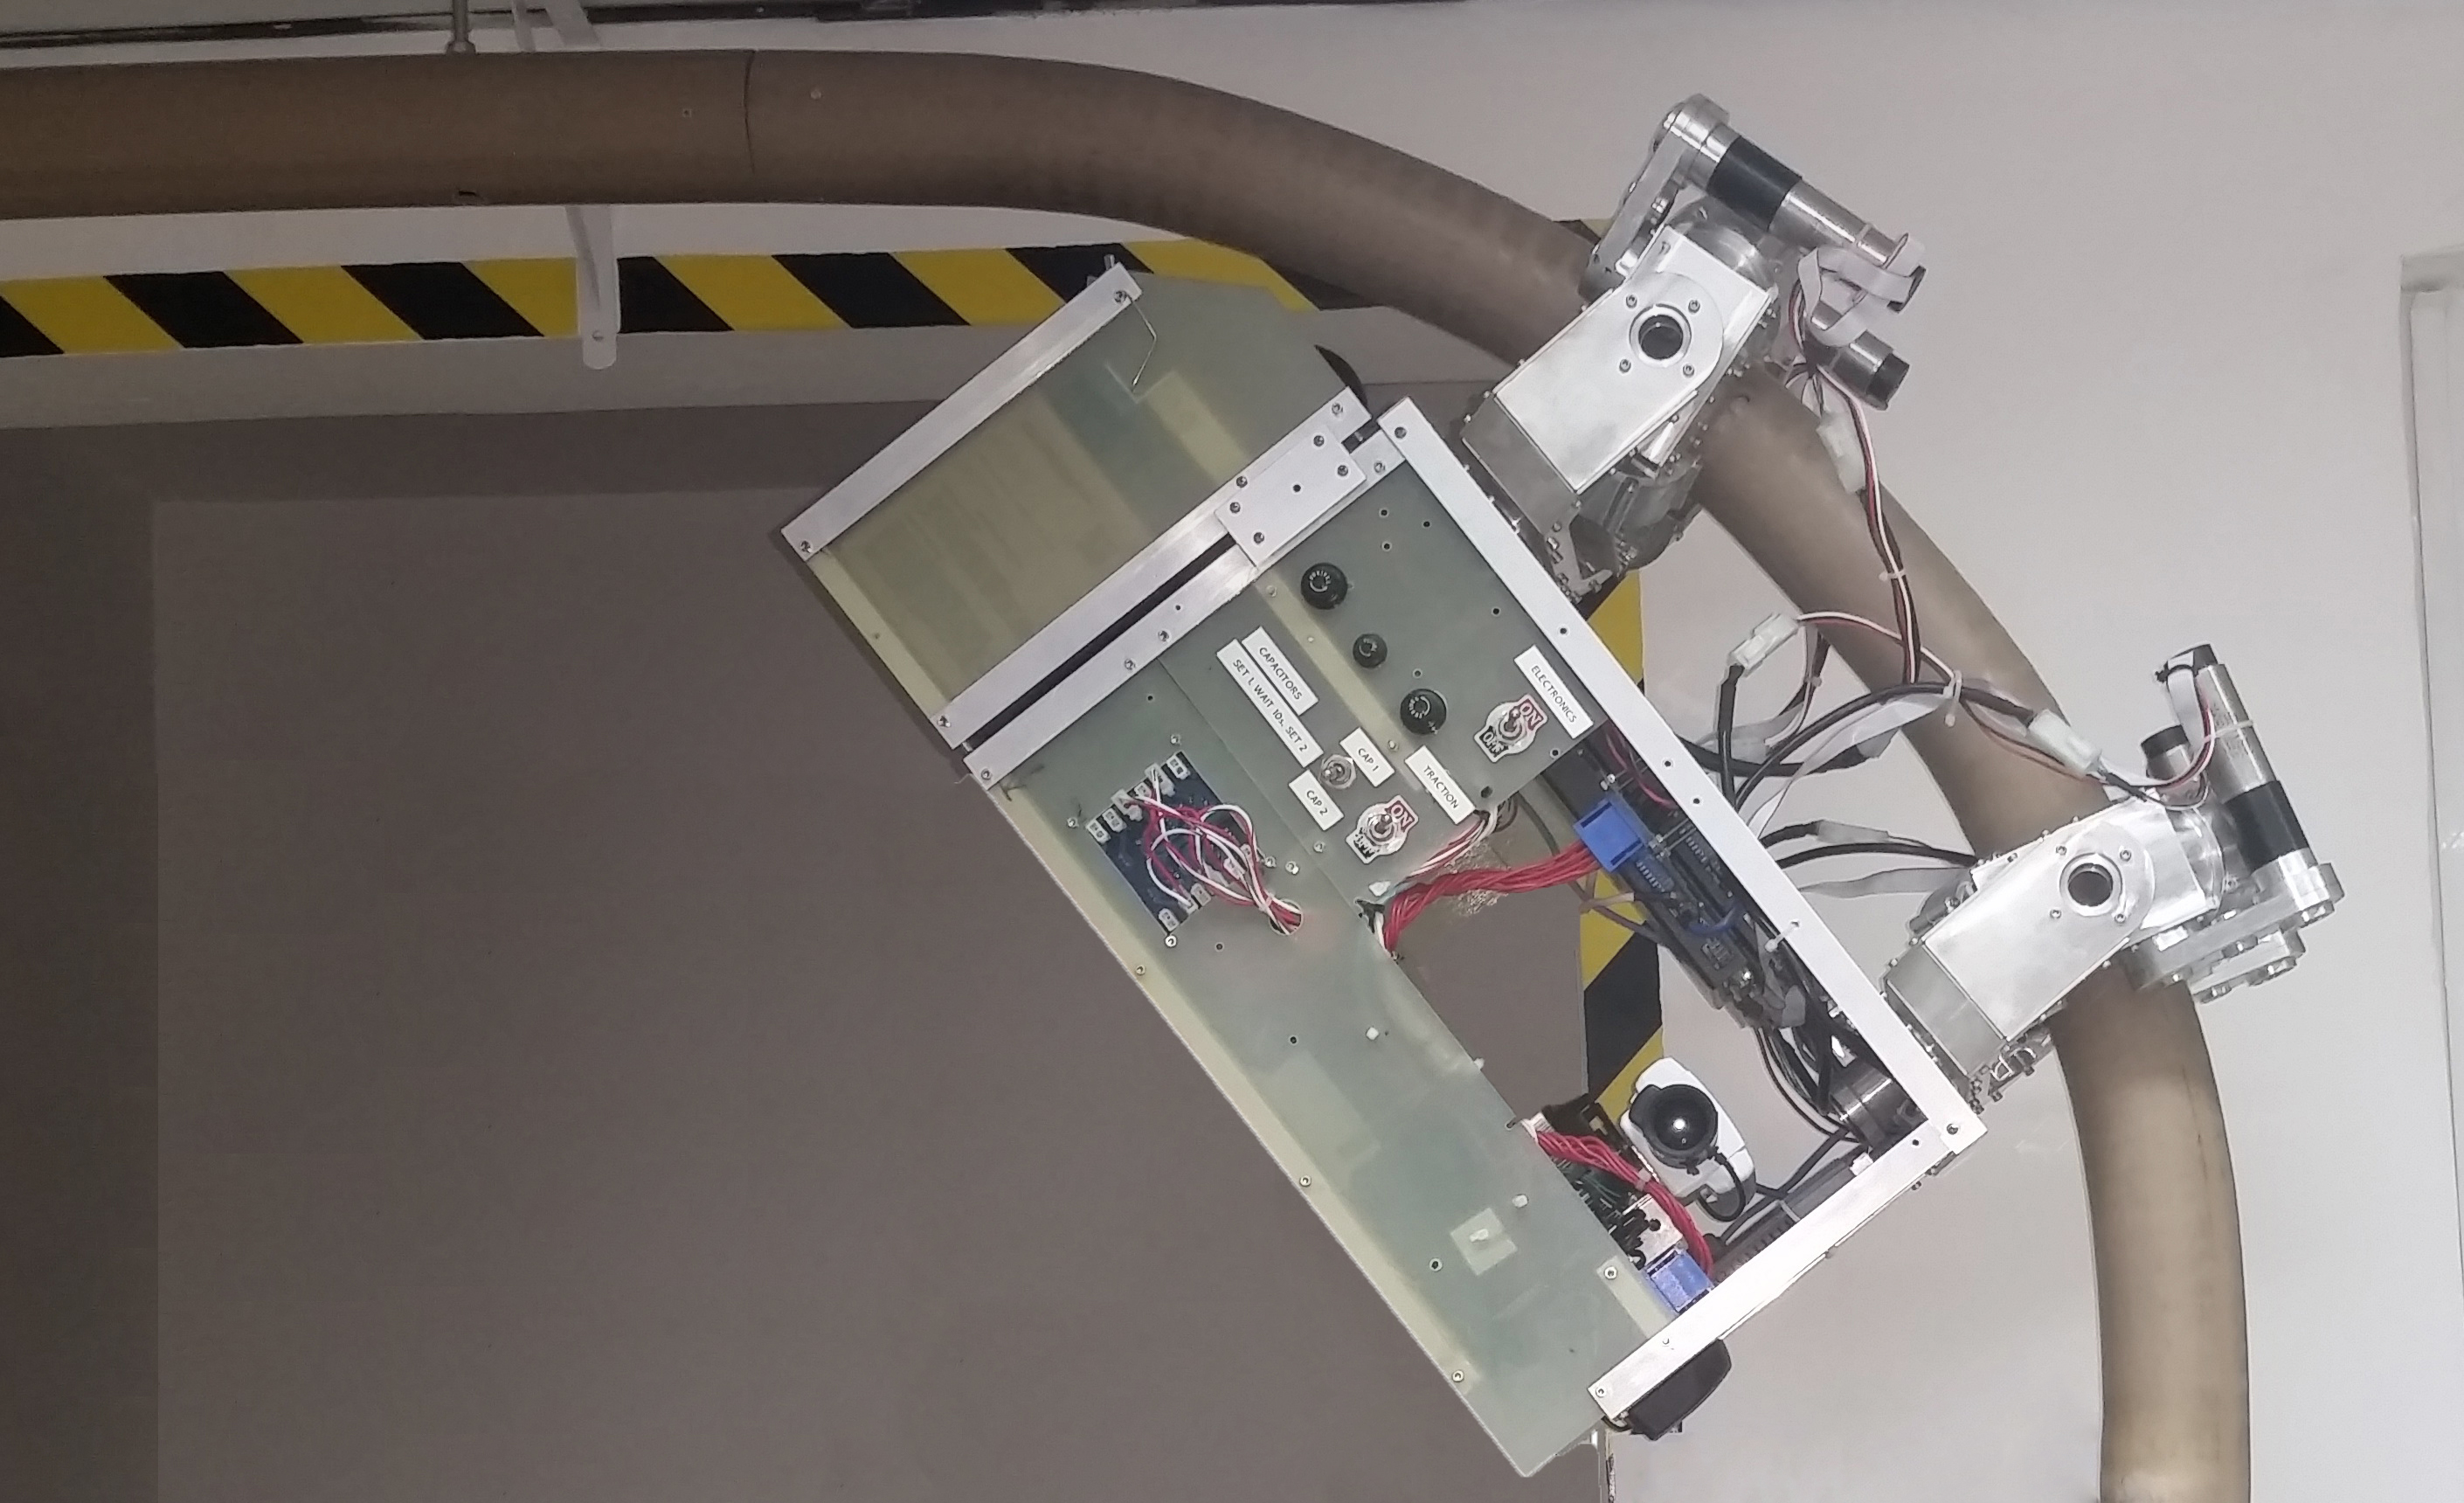
\includegraphics[width=8.4cm]{figs/SAM5.jpg}
\caption{SAM - Single Autonomous Module.}
\label{fig:SAM2}
\end{figure}

The communication system was implemented as the following: an \emph{Ethernet
communication network} to connect the fixed camera, the computer, and the access
point; a \emph{Wi-Fi communication network} to connect SAM with the operation
base; a \emph{CAN bus} to control the actuators; and two stereoscopic
Webcams and IMU were plugged to the computer through USB connections. The robot operation range is
limited to the Wi-Fi antenna, and, to improve it Wi-Fi,
repeaters and intrinsic safe barriers should be installed.
To ensure data loss prevention, all data is firstly stored and processed
locally, and then transmitted.

The concept of independent power buses proved to be efficient, and the designed
battery capacity could handle the system energy demand. The robot autonomy was
greater than five hours, but it will highly depend on the embedded devices, the
required task and the rail track. It was observed that when SAM moves
downwards, the motors control brake the robot, generating a brake energy on the
way back to the source. Depending on the length of the downhill section, and on
the robot's speed, this energy may reach a voltage level that causes the motors
drivers to reset.
%This issue must be further studied to
%investigate if it is worth to store this extra energy or simply waste it using
% an additional device to dissipate this energy as heat.

Furthermore, it was verified that SAM can be teleoperated from anywhere by
accessing its Wi-Fi network and the GUI developed in Qt environment. SAM has
already been teleoperated by Petrobras (from Brazil) and by Statoil (from Norway). The robot performed position and
velocity tracking tasks and the video camera frames were sent from Brazil and
received in Norway with a two seconds delay. As the main goal of DORIS is to
have autonomous capabilities and to be operated locally in the offshore
platform, delays due to distance souldn't be of major concern.

\subsection{Vehicle Support System (VSS) Tests}\label{sec:VSS_tests}
All DORIS VSS functions were successfully tested independently. The AVR firmware was programmed in C++ using Atmel Studio 6.1.
The following tests/implementations were successfully performed:
\begin{enumerate}[i)]
    \item Logic to command the \emph{solid-state relays} to turn on/off some devices;
    \item Acquisition of \emph{module voltages} and \emph{module currents}:
    DC-DC voltage (5, 12 and 24 Vdc), battery raw voltage measurements, and the
    currents that supply each device;
    \item Acquisition of \emph{module temperature/humidity};
    \item Acquisition of \emph{battery information} through SMBUS: voltage,
    temperature, current, state of charge, and battery status;
    \item \emph{Timers} to enable robot shutdown in predetermined time, and
    periodic data report of voltages, currents, relays status, temperature, and
    humidity;
    \item \emph{Ethernet Communication}: all data can be accessed via Ethernet.
\end{enumerate}

\section{Conclusion and Future work}\label{sec:conclusions}

In this paper, we presented the EE and software architecture
of the DORIS project, which endeavors to develop an offshore facilities
inspection and monitoring robot. All the mobile offshore robots seen so far are
wheeled robots,  which enables great flexibility and a large inspection area. However,
they have to deal with complex problems compounded by the offshore platform environment,
such as autonomous navigation, mobility, and collision avoidance. DORIS uses a
rail for motion as a tradeoff between constrained mobility and alleviation of
of the above issues. It has an onboard electronics with multiple fail safes,
power management, and a state of the art vehicle support system.

%The prototype is based on rail guided modules powered by a battery system and equipped with multiple
%sensors that enable the detection of anomalies, such as abandoned objects and
%gas leakage.

A prototype, SAM, was built to test the electronics, power supply, and software
architecture concepts.
Preliminary results show good overall performance of sensor integration and
communication, independent power buses for electronics and motors, and
teleoperation.

The Vehicle Support System was tested in a simple testing platform, and the
customized PCBs were able to monitor temperature/humidity, DC-DC
voltage levels, the devices' currents, and batteries data via SMBUS.
%The solid-state relays can also turn on/off the devices for protection and/or
%efficiently power consumption.

Ongoing implementations and future challenges include:
\begin{enumerate}[i)]
 
  \item \emph{New VSS tests}:
  implementation of the BMS logic that uses the SMBUS data to manage energy distribution;
  %\item \emph{Expansion and reconfiguration of robot modules}:\\
  %DORIS will need more than one module to support all the defined devices and
  % features.
  %The EE system permits the free expansion and reconfiguration of DORIS
  % modules, enabled by the bus topology for DORIS main networks: Ethernet and CAN.
  \item \emph{Autonomous operation}: advanced localization, mapping, and
  mission control;
  %The
  %Positioning System, which currently comprises wheels' encoders (odometry), a
  %fixed camera (3D mapping), and an inertial movement unit
  %(IMU) will be upgraded with the detection of rail landmarks, such as rail
  %supports and segments connections. The fusion of these measurements will help
  %to estimate the vehicle states, such as position, attitude and velocity;
  \item \emph{Reduced interferences}:
  An electrostatic discharger should be designed to drain the accumulated
  charge from the shielding system;
  \item \emph{Solution for DORIS downhill motion issue}: Tests will be held to measure the generated amount of energy to decide
  if it is worth to store or waste it;
  \item \emph{Hardware Certification}: 
  DORIS must be certified to operate in harsh and explosive environments.
\end{enumerate}

\bibliography{ifacconf}

\appendix

\end{document}